\section{Protocolo IPv6}

A medida que avanzaba el tiempo, las direcciones IPv4 escaseaban, habían tablas de ruteo muy grandes y mucha congestión entre los routers por exceso de procesamiento. Por esto se introduce un protocolo nuevo: IPv6.


\subsection{Cambios con respecto a IPv4}

Los aspectos modificados son los siguientes:

\begin{itemize}[label=\textcolor{acento}{$\bullet$}]
    \item Direcciones de 128 bits.
    \item No hay más fragmentación.
    \item No hay más header checksum.
    \item El header es de tamaño fijo, sin campo de opciones.
    \item Se extiende el protocolo con cabeceras de extensión.
\end{itemize}

\begin{figure}[htbp]
    \centering
    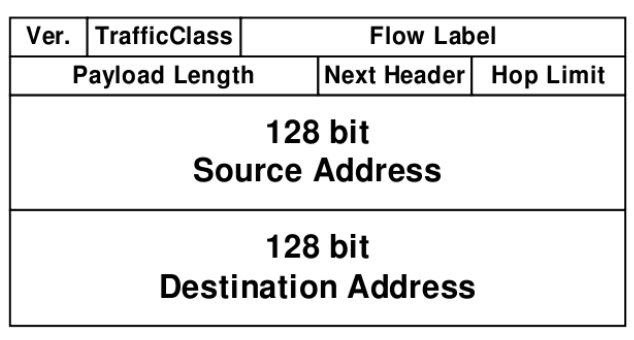
\includegraphics[width=0.5\textwidth]{capitulos/ipv6/imagenes/header-ipv6.png}
    \caption{Header de IPv6}
    \label{fig:header-ipv6}
\end{figure}


\subsection{Direcciones IPv6}

También se modifican los tipos de direcciones: ya no hay direcciones de broadcast, sino que hay unicast, anycast y multicast, que tienen formato \texttt{FF00::/8}.

La notación cambia. Los ceros al inicio de cada grupo de 2 bytes delimitados por \texttt{:} se pueden obviar, como también los ceros contiguos con \texttt{::}, aunque este se puede utilizar una sola vez por dirección.

Tampoco existe la máscara de red, ya que el prefijo es /64 para las subredes y los link-local. La dirección de loopback ahora es \texttt{::1/128}.